\documentclass[italian]{report}
\usepackage{graphicx}
\usepackage{booktabs}
\usepackage{geometry}
\usepackage{hyperref}
\usepackage{babel}
\usepackage{lipsum}

 \geometry{
 a4paper,
 total={170mm,257mm},
 left=20mm,
 top=20mm,
 }

\title{
    \leavevmode{
\includegraphics[width=1\textwidth]{../resources/img/polito_logo_2021_blu}\newline\newline}\\
     Fingerprint spoofing detection \\

}
\author{Riccardo Cardona, Nicholas Berardo}

\begin{document}

\maketitle

\chapter{Introduzione}
\lipsum[1]

\chapter{Classification and Validation}

\section{Introduzione}

\section{Multivariate Gaussian Classifiers}

\begin{table}[h!]
    \centering
    \begin{tabular}{@{}llll@{}}
    \hline
    Classifier          & pi = 0.1  & pi = 0.5  & pi = 0.9 \\ \hline
                        & \multicolumn{3}{c}{RAW Features} \\
    Gaussian            & 0.593     & 0.333     & 0.111    \\
    Naive Gaussian      & 0.815      & 0.47     & 0.146    \\
    Tied Gaussian       & 0.722     & 0.484     & 0.185    \\
    Naive Tied Gaussian & 0.794     & 0.564     & 0.203    \\ \hline
    \end{tabular}\label{tab:table}
\end{table}

\begin{table}[h!]
    \centering
    \begin{tabular}{@{}lllllll@{}}
    \toprule
    Classifiers         & pi = 0.1 & pi = 0.5 & pi = 0.9 & pi = 0.1   & pi = 0.5   & pi = 0.9  \\ \midrule
                        & \multicolumn{3}{c}{PCA (m=5)}  & \multicolumn{3}{c}{PCA + LDA (m=5)} \\
    Gaussian            & 0.652    & 0.354    & 0.112    & 0.652      & 0.354      & 0.112     \\
    Naive Gaussian      & 0.912    & 0.446    & 0.122    & 0.732      & 0.402      & 0.13      \\
    Tied Gaussian       & 0.685    & 0.501    & 0.192    & 0.685      & 0.501      & 0.192     \\
    Naive Tied Gaussian & 0.905    & 0.681    & 0.218    & 0.685      & 0.501      & 0.192     \\ \bottomrule
    \end{tabular}\label{tab:table2}
\end{table}

\begin{table}[h!]
    \centering
    \begin{tabular}{@{}lllllll@{}}
    \hline
    Classifiers         & pi = 0.1 & pi = 0.5 & pi = 0.9 & pi = 0.1   & pi = 0.5   & pi = 0.9  \\ \hline
                            & \multicolumn{3}{c}{PCA (m=8)}  & \multicolumn{3}{c}{PCA + LDA (m=8)} \\
    Gaussian            & 0.604    & 0.338    & 0.111    & 0.604      & 0.338      & 0.111     \\
    Naive Gaussian      & 0.869     & 0.43    & 0.118    & 0.669      & 0.405      & 0.145     \\
    Tied Gaussian       & 0.711    & 0.484    & 0.183    & 0.711      & 0.484      & 0.183     \\
    Naive Tied Gaussian & 0.912    & 0.671    & 0.213    & 0.711      & 0.484      & 0.183     \\ \hline
    \end{tabular}\label{tab:table3}
\end{table}

\newpage

\section{Logistic Regression}
The plots show how minDCF is affected by different values of $\lambda$.  They are exploited to calibrate
$\lambda$, which is the regularization term.

\begin{figure}[h!]
    \centering
    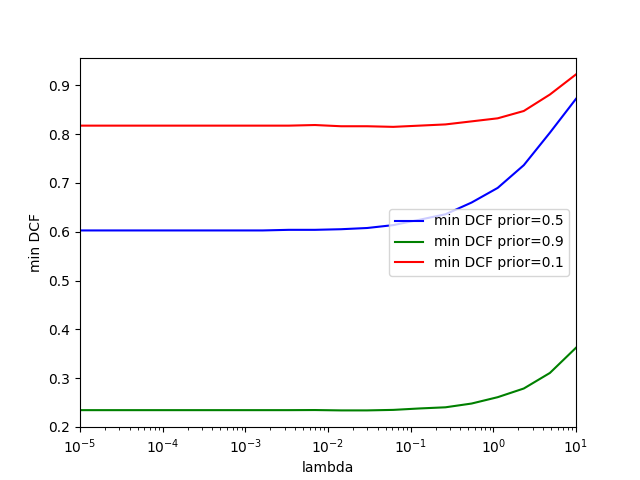
\includegraphics[scale=0.5]{../../images/DCF_LR, LR_minDCF_comparison.png}
    \caption{DCF - RAW LogReg}
    \label{DCF - RAW LogReg}
\end{figure}

\end{document}